\documentclass[11pt]{article}
\usepackage{fancyheadings,multicol}
\usepackage{amsmath,amssymb}
\usepackage{graphicx}
\usepackage{caption}
\usepackage{subcaption}
\usepackage{hyperref}
\usepackage[]{algorithm2e}
\usepackage{graphicx}
\usepackage{hyperref}
\usepackage{diagbox}

%% Custom page layout.
\setlength{\textheight}{\paperheight}
\addtolength{\textheight}{-2in}
\setlength{\topmargin}{-.5in}
\setlength{\headsep}{.5in}
\addtolength{\headsep}{-\headheight}
\setlength{\footskip}{.5in}
\setlength{\textwidth}{\paperwidth}
\addtolength{\textwidth}{-2in}
\setlength{\oddsidemargin}{0in}
\setlength{\evensidemargin}{0in}
\flushbottom

\allowdisplaybreaks




%% Custom headers and footers.
\pagestyle{fancyplain}
\let\headrule=\empty
\let\footrule=\empty
\lhead{\fancyplain{}{Chao Tao, Yangchen Pan}}
\rhead{\fancyplain{}{CSCI-B555: Machine Learning}}



\begin{document}

\thispagestyle{plain}

\begin{center}
\bfseries
{\Large Class Project: Rossmann Store Sales Prediction}\\
   Student Name(s): Chao Tao, Yangchen Pan\\
   \today
\end{center}

\textbf{Introduction:} This project is chosen from Kaggle competition website, aiming at predicting $1115$ stores' sales across $7$ European countries by exploring the sales data from 01/01/2013 - 07/31/2015. Our team carefully examined the data set and make a significant improvement in the training set by feature transformation and creation. We then applied roughly $10$ machine learning algorithms to do prediction, based on our exploratory analysis on the training and testing set. An ensemble method was finally applied and its prediction results serve as the final submission. 

\section{Task Allocation}
Chao Tao: data set exploratory analysis, feature transformation and creation, data set splitting design, self-implemented stochastic kernel linear regression, ensemble method design, ridge regression, linear regression, bayes regression, support vector regression.   

Yangchen Pan: data set exploratory analysis, feature transformation and creation, data cleaning, self-implemented algorithm 1 (described below), regularizer selection, ensemble method design, poisson regression, regular kernel regression with different kernels, etc.

Summary: cooperate well without caring much about task weights.   
\section{Description of dataset}

Data set source: \hyperref[Rossmann Store Sales]{https://www.kaggle.com/c/rossmann-store-sales/data}
\\

In this project, we have totally $4$ files, i.e. ``train.csv", ``test.csv", ``sample\_submission.csv" and ``store.csv". Our aim is to predict daily sales for $1115$ stores. In table ``store.csv", there are totally $10$ attributes. This table provides supplemental information about stores. 
\begin{table}[ht!]
	\begin{center}
		\begin{tabular}{|l|p{8cm}|}
			\hline
			Attribute & Description \\
			\hline
			StoreType & Differentiates between 4 different store models: a, b, c, d \\
			\hline
			Assortment & Describes an assortment level: a=basic, b=extra, c=extended \\
			\hline
			CompetitionDistance & Distance in meters to the nearest competitor store\\
			\hline
			CompetitionOpenSinceMonth & Gives the approximate month of the time the nearest competitor was opened\\
			\hline
			CompetitionOpenSinceYear & Gives the approximate year of the time the nearest competitor was opened\\
			\hline
			Promo2 & Promo2 is a continuing and consecutive promotion for some stores: 0 = store is not participating, 1 = store is participating\\
			\hline
			Promo2SinceWeek & Describes the calendar week when the store started participating in Promo2\\
			\hline
			Promo2SinceYear & Describes the year when the store started participating in Promo2\\
			\hline
			PromoInterval & Describes the consecutive intervals Promo2 is started, naming the months the promotion is started anew. E.g. ``Feb,May,Aug,Nov" means each round starts in February, May, August, November of any given year for that store\\
			\hline
		\end{tabular}
	\end{center}
	\caption{store.csv}
	\label{table1}
\end{table}%

In table ``train.csv", there are totally $9$ attributes. This table provides historical data including Sales. 

\newpage
\begin{table}[ht!]
	\begin{center}
		\begin{tabular}{|l|p{8cm}|}
			\hline
			Attribute & Description \\
			\hline
			Store & A unique Id for each store which is from $1$ to $1115$ \\
			\hline
			DayOfWeek & Indicates which day of a week\\
			\hline
			Date & Data information like ??/??/????\\
			\hline
			Sales & The turnover for any given day (this is what we are predicting)\\
			\hline
			Customers & The number of customers on a given day\\
			\hline
			Open & An indicator for whether the store was open: 0 = closed, 1 = open\\
			\hline 
			Promo & Indicates whether a store is running a promo on that day\\
			\hline
			StateHoliday  & Indicates a state holiday. Normally all stores, with few exceptions, are closed on state holidays. Note that all schools are closed on public holidays and weekends. a = public holiday, b = Easter holiday, c = Christmas, 0 = None\\
			\hline
			SchoolHoliday & Indicates if the (Store, Date) was affected by the closure of public schools\\
			\hline  
		\end{tabular}
	\end{center}
	\caption{train.csv}
	\label{table2}
\end{table}%

In table ``test.csv", there are totally $9$ attributes. This table without Sales and Customers is similar with ``train.csv" except using another Id that represents a (Store, Date) duple within the test set. Therefore, similar to ``sample\_submission.csv", our predicting table should consist of two attributes, i.e. ``Id" and ``Sales". 


\section{Data Preprocessing}

\subsection{Features Transformation}

Observing that some features of a store should be also meaningful to predict sales, we merged the $stores.csv$ and the $train.csv$ files first.  

First, to decrease data set size, we deleted the rows where the store does not open or sales is zero, which is not useful for our prediction. Second, observing there is a date column, which cannot be directly used for analysis purpose, we separate the date column to two columns: month index in a year and day index in a month. By this transformation, we assumed the sales show some periodic relationships with the relative time in a year and in a month. Third, we transform a discrete variable with more than $2$ categories to multiple binary features, make it convenient to compute distance between different examples. Fourth, we create new columns (features) by using multiple existed columns to make the feature easier to handle. For example, for the column Promo2Since(Year/Week), which describes the year and calendar week when the store started participating in Promo2, we transformed it to how long it has been participating in Promo2. Another example is, for the column PromoInterval, which describes the consecutive intervals Promo2 is started, naming the months the promotion is started anew. We convert it to a binary feature which denotes whether the current store at current date is in this interval. For the \emph{DayOfWeek} feature, we convert it to six dummy variables. To handle the variance in week index in a month, we also create four dummy features to denote which week the current date is in the context of the current month. Two lists below shows comparison between features before and after transformation. Please see the appendix to check the code for data preprocessing. 
\\
\\
\textbf{Features before preprocessing}: \\
DayOfWeek, Date, Open, Promo, StateHoliday, SchoolHoliday, StoreType, Assortment, CompetitionDistance, CompetitionOpenSinceMonth, CompetitionOpenSinceYear, Promo2, Promo2SinceWeek, Promo2SinceYear, PromoInterval
\\
\\
\textbf{Features after preprocessing}:\\
Promo, StateHoliday, SchoolHoliday, MonthInYear, Promo2Duration, CompDuration	InPromoInterval, Day\_1, Day\_2, Day\_3, Day\_4, Day\_5, Day\_6, Month\_8, Month\_9, WeekM\_1, WeekM\_2, WeekM\_3, WeekM\_4

\subsection{Dataset Splitting}

One should notice that the provided testing set has no sales column so we should totally use the training set as the whole data set to do model design and evaluation. 
\\

Depending on different types of algorithm, we have different splitting methods. Since we train multiple models for each store, what we do is to split the original training set to three parts: one training set, one validation set and one testing set. The validation set is to do model selection. Due to our particularly designed algorithm, we split the training data set to a new training set and testing set, since the sales values are not available in the originally provided testing set. One thing worth mentioning is that, the customers column in the original training data set is not provided in the testing set since we cannot know the customers in advance, so I set two prediction targets for my algorithm, one is number of customers and another one is sales. You will see how I utilize this two targets to do prediction. Another important change worth mentioning is that, in the observance of the test set only has month $8$ and $9$, when I split the current training set, I only set those rows with month $8$ and $9$ and year $2014$ as the validation set to do evaluate model before submission. 

\section{Description of methods}

\subsection{Why we firstly choose kernel regression}

We first think of kernel regression after carefully reviewing this prediction problem. This intuition comes from the observance of the time series pattern of sales data. The sales for a certain store kind of repeat some patterns through the whole year. By using kernel regression, new representation can be derived from comparing the similarity between current new example to some past example, in which way we can emphasize the importance of different date by including some non-trivial time data in our training set. You can see this effort from the previous part about feature transformation.  

\subsection{Algorithms}

We tried linear regression, ridge regression, lasso regression, support vector regression with linear and polynomial kernel, kernel linear regression, poisson regression, bayes regression, and stochastic optimization for kernel regression. We also designed a particular algorithm to solve this prediction problem. However, due to the long training time for our algorithm, we only use a regular ensemble method to do prediction as the final submission result. Below are the most important and effective algorithms implemented by ourselves to do predictions. 
\\
First, our self-designed algorithm borrows idea from EM algorithm. Observing that there is a column of number of customers in the training set, but there is no such column in the testing set, I still try to use it during the training process. Basic idea is to predict customers first, then use the predicted results to predict sales; then discard the customers and use the data set with the predicted sales to do prediction. The algorithm requires an separate validation set to see whether the prediction error no longer changes much. This algorithm takes a relatively long time to finish predictions. Especially for the given data set, there are more than $1000$ stores and we will train the model on each store to do prediction. The find-center function below can be some clustering algorithm and can also be some random samples from training set. Please see appendix for this part of code due to the significant amounts. 
\\
Notations for $algorithm-1$: \\
Training set: $\mathbf{D}$;\\
Testing set without sales and customers: $\mathbf{N}$;\\
$\mathbf{T}$: training data split from $\mathbf{D}$; \\
$\mathbf{V}$: validation data split from $\mathbf{D}$; \\
$\mathbf{X}, \mathbf{yc}, \mathbf{ys}$ respectively: features, customers target, sales target split from $\mathbf{T}$;\\
$\mathbf{vX}, \mathbf{vyc}, \mathbf{vys}$: features, customers target, sales target split from $\mathbf{V}$.

\newpage
\begin{algorithm}[ht]
	\KwData{Input: training set, $\mathbf{D}$; testing set without sales and customers, $\mathbf{N}$}
	\KwResult{Prediction sales for $\mathbf{N}$}
	\While{store index i in index range:}{
		read $\mathbf{N}, \mathbf{D}$ with store index i \;
		$\mathbf{T}, \mathbf{V} := \mathbf{D}$\;
		$\mathbf{X}, \mathbf{yc}, \mathbf{ys} := \mathbf{T}$\;
		$\mathbf{vX}, \mathbf{vyc}, \mathbf{vys} := \mathbf{V}$\;
		centers\_c = find-centers($\mathbf{X}, \mathbf{yc}$)\;
		centers\_s = find-centers($\mathbf{X}, \mathbf{ys}$)\;
		centers = find-centers($\mathbf{X}$)\;
		olderror = infinity\;
		error = infinity\;
		error\_dif = infinity\;
		\While{error\_dif $ < threshold$}{
			pass\_in\_centers = choosefrom(centers\_c,centers\_s,centers)\;
			pass\_in\_target = choosefrom($\mathbf{yc}, \mathbf{ys})$\;
			model = kernel\_regression($\mathbf{X}, pass\_in\_target, pass\_in\_centers$) \;
			$\hat{\mathbf{yc}} = model.predict(\mathbf{N}$)\;
			$\mathbf{N} := combine(\mathbf{N}, \hat{\mathbf{yc}})$ \;
			
			$\mathbf{vX} := combine(\mathbf{vX}, \hat{\mathbf{vyc}})$ \;
			$\hat{\mathbf{vyc}} = model.predict(\mathbf{vX}$)\;
			$olderror = error$\;
			$error = geterror(\hat{\mathbf{vyc}}, \mathbf{vyc})$\;
			$\mathbf{vX} := remove(\mathbf{vX}, \mathbf{vyc})$\;
			$\mathbf{vX} := combine(\mathbf{vX}, \hat{\mathbf{ys}})$ \;
			
			$\mathbf{X} := combine(\mathbf{X}, \mathbf{yc})$ \;
			$model = kernel\_regression(\mathbf{X}, pass\_in\_target, pass\_in\_centers)$ \;
			
			$\hat{\mathbf{ys}} = model.predict(\mathbf{N}$)\;
			$\mathbf{N} := remove(\mathbf{N}, \hat{\mathbf{yc}})$ \;
			$\mathbf{N} := combine(\mathbf{N}, \hat{\mathbf{ys}})$ \;
			$\mathbf{X} := remove(\mathbf{X}, \mathbf{yc})$\;
			$\mathbf{X} := combine(\mathbf{X}, \mathbf{ys})$\;
			
			$error\_dif = abs(error - olderror)$\;
		}{
	 return $\hat{\mathbf{ys}}$\;
	}
}
\caption{Self-designed kernel regression}
\end{algorithm}

Second, we implemented a stochastic gradient descent algorithm for kernel linear regression. The basic idea is just to perform stochastic gradient descent on new representation of original data set. Below are the core part of code. The basic idea is, for each sample, we scan all chosen centers to generate a new representation for that sample; then we can use this new sample to perform gradient descent. 

\begin{verbatim}
def sgdlearn(self, Xtrain, ytrain, kerneltype = "linear", regularizer = 10, numofpasses = 2):
    self.kerneltype = kerneltype
    stepsize = 0.00000001
    self.weights = np.random.rand(self.centers.shape[0]+1)
    for i in range(numofpasses):
        for exid in range(Xtrain.shape[0]):
        kernelrep_exid = list(map(self.polynomialkn,...
        np.repeat(np.array([list(Xtrain[exid,:])]),
        len(self.centers),axis=0),self.centers))
        kernelrep_exid.append(1)
        kernelrep_exid = np.array(kernelrep_exid)
        print(exid)
        self.weights = self.weights - stepsize * ...
        ( np.dot(np.dot(kernelrep_exid, self.weights)...
        -ytrain[exid], kernelrep_exid)+ regularizer * self.weights)
        #print(self.weights)
    print(list(self.weights))
    
def sgdpredict(self, Xtest):
   ytest = []
   for xi in Xtest:
      kernelrep_exid = list(map(self.polynomialkn, ...
      np.repeat(np.array([xi]),len(self.centers),axis=0),self.centers))
      kernelrep_exid.append(1)
      kernelrep_exid = np.array(kernelrep_exid)
      ytest.append(np.dot(self.weights,kernelrep_exid))
   return ytest
\end{verbatim} 

Third, due to the bad accuracy from SGD on kernel regression, and the long running time of our first algorithm, we use a simpler ensemble method to do prediction as the submission. The basic idea is to use three different types of kernels along with a regular linear regression, bayes regression, Poisson regression, support vector linear kernel regression, support vector polynomial kernel regression, and then linearly combine the best five models with different weights to get an ensemble prediction. To verify Poisson regression is reasonable here, I carefully examined the distribution of sales for several random stores as below figure shows\ref{fig:figure1} and \ref{fig:figure2}. Another reasonable motivation of using Poisson regression here is that the sales target is integer. The ensemble algorithm is below. Note: this algorithm does not use the customers column.

\newpage
\begin{algorithm}[ht]
	\KwData{Input: training set, $\mathbf{D}$; testing set without sales, $\mathbf{N}$}
	\KwResult{Prediction sales for $\mathbf{N}$}
	\While{store index i in index range:}{
		Get corresponding data set with store index i from $\mathbf{D}, \mathbf{N}$\;		
		$\mathbf{T}, \mathbf{V} := \mathbf{D}$\;
		$\mathbf{X}, \mathbf{ys} := \mathbf{T}$\;
		$\mathbf{vX}, \mathbf{vys} := \mathbf{V}$\;
		Using $\mathbf{X}, \mathbf{ys}$, do\;
		$M_1$ := Train linear kernel regression model\;
		$M_2$ := Train poly kernel regression model\;
		$M_3$ := Train gaussian kernel regression model\;
		$M_4$ := Train linear regression model\;
		$M_5$ := Train bayes regression model\;
		$M_6$ := Train Poisson regression model\;
		$M_7$ := Train Support vector regression with linear kernel\;
		$M_8$ := Train Support vector regression with poly kernel\;
		Using $\mathbf{vX}, \mathbf{vys}$, do\;
		$error_1$ := geterror($M_1$)\;
		$error_2$ := geterror($M_2$)\;
		$error_3$ := geterror($M_3$)\;
		$error_4$ := geterror($M_4$)\;
		$error_5$ := geterror($M_5$)\;
		$error_6$ := geterror($M_6$)\;
		$error_7$ := geterror($M_7$)\;
		$error_8$ := geterror($M_8$)\;
		Get the index set $\mathcal{I}, |\mathcal{I}| = 5$ with lowest errors\;
		For each $M_i, i \in \mathcal{I}$, computing weight $w_i$\;
		$$w_i = \frac{1/error_i}{\sum_{i=1}^{5} \frac{1}{error_i}}$$
		Train $M_i$ on the original training data set $\mathbf{D}$\;
		$\hat{\mathbf{ys}} = \sum_{i = 1}^{5} w_i M_i.predict(\mathbf{N})$\;
		store $\hat{\mathbf{ys}}$ for submission\;
		}{
		return\;
	}
\caption{Ensemble Prediction}
\end{algorithm}

\newpage
\begin{figure}[ht]
	\centering
	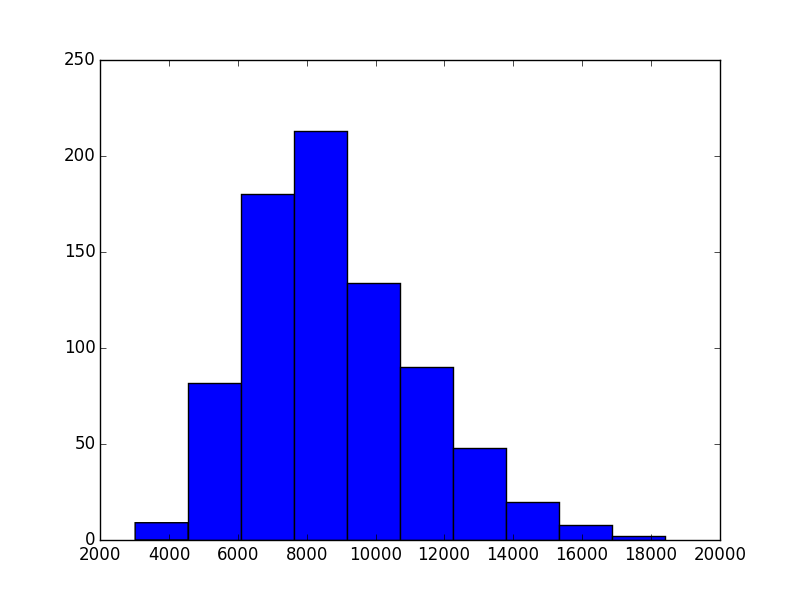
\includegraphics[scale = 0.5]{sales_histogram1}
	\caption{Sales Distribution: store 3 \label{fig:figure1}}
\end{figure}

\begin{figure}[ht]
	\centering
	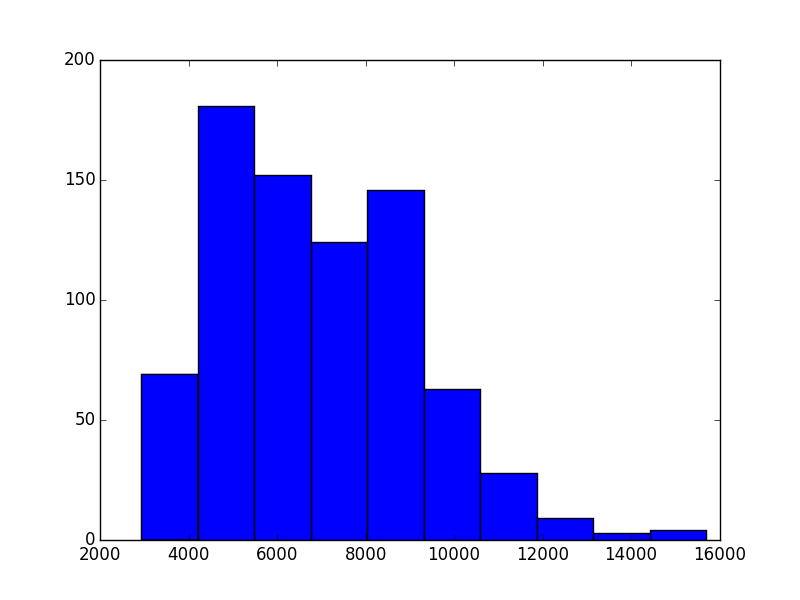
\includegraphics[scale = 0.5]{sales_histogram2}
	\caption{Sales Distribution: store 7 \label{fig:figure2}}
\end{figure}

\newpage

\subsection{Parameter Selection}

The most important parameters here to select include: regularizer, number of centers and polynomial degree in poly-kernel function, and the variance parameter in Gaussian kernel function. Polynomial degree and variance parameter are selected simply by random test, since we want to fix some parameters to better select other parameters. By using systematic test, the number of centers is directly fixed as the number of training examples. So the last thing to do is to decide the regularizers, which is really important from our experiments. 

Fix one regularizer, we observe the significant difference on the performance of predicting sales for each store. Then I examined the variances of different stores' sales and print out the statistics of all the variances. The result is in \emph{variances.txt} file. Then I selected the $0.2, 0.4, 0.6, 0.8$ four percentiles to divide those variances to four levels. Selecting regularizer is based on how large the variance of the current store's sales is. The assumption is: \textbf{Large variances on target variable corresponds to large variances on the features, consequently, we want to choose relatively larger regularizer for the training set with large variance of target variable}. The concrete function is below. Those cutoff numbers in the function correspond to those percentiles of variance mentioned above. 

\begin{verbatim}
def chooseregularizer(v):
   if v <= 331721:
      return 0.00000001
   elif v<= 1762504:
      return 0.00000002
   elif v<=2635979:
      return 0.00000004
   elif v<=3652159:
      return 0.00000006
   elif v<=5149050:
      return 0.00000008
   else:
      return 0.01
\end{verbatim}%

\section{Results}

The model evaluation method written in script\_classify.py is an implementation of the criteria required by the competition problem website, which is Root Mean Square Percentage Error (RMSPE). The formula is: $$RMSPE = \sqrt{\frac{1}{n} \sum_{1}^{n} (\frac{y_i - \hat{y_i}}{y_i})^2}.$$ With $11$ submission times, we current get the RMSPE $0.13237$, and the current lowest error is $0.08949$ and current highest error is $0.99983$. We randomly select three stores' prediction results through table~\ref{table:table3}. One can easily observe that different algorithms can have significant performance on predicting different stores. 

\begin{table}
	\centering
	\label{table:table3}
	\begin{tabular}{|p{3.15cm}|c|c|c|}
		\hline
		\diagbox{Method}{Error}{Store Id} & 245 & 247 & 248 \\
		\hline
		SVM polynomial kernel regression & 0.1646 & 0.1270 & 0.1277 \\
		\hline
		SVM linear kernel regression & 0.1200 & 0.1129 & 0.1041 \\
		\hline
		linear kernel regression & 0.1121 & 0.1077 & 0.1014 \\
		\hline
		poisson kernel regression & 0.1980 & 0.1006 & 0.1553 \\
		\hline
		gaussian kernel regression & 0.1866 & 0.1054 & 0.1385 \\
		\hline
		linear regression & 0.1120 & 0.1081 & 0.1015 \\
		\hline
		bayes regression & 0.1100 & 0.1064 & 0.1051 \\
		\hline
		poisson regression & 0.1118 & 0.1080 & 0.1018 \\
		\hline
	\end{tabular}
	\caption{Prediction error of some stores under different regression methods}
\end{table}


\subsection{Algorithm selection}

First, let me summarize the framework of how the prediction is performed. \textbf{Every algorithm} we described above is applied within the below framework. As a result, instead of using cross validation on training set to do model comparison, we directly use different stores to do prediction to evaluation our models. The self-designed algorithm here is also unstable and sometimes cannot converge. The most important disadvantage is it takes long time to train the mode. The concrete model comparison method can be using statistical testing as the assignment $4$ does. We finally choose the result of the ensemble method as the final submission with the consideration of accuracy and time complexity.  

\begin{algorithm}[H]
	\KwData{Input: training set and provided testing set}
	\KwResult{Prediction sales for provided testing set}
	\While{store index i in index range:}{
	 update the training set as those with store index i\;
	 update the testing set as those with store index i\;
     Apply some algorithms\;
     Write prediction output to file for store i\;
	}
	return\;
\caption{Prediction Framework}
\end{algorithm}

Run the algorithm(s) and variants in a exploratory experimental analysis.
The goal here is to try to conclude what algorithm you would submit
to the competition. To do so requires a reasonable experimental design where you can
draw some conclusions about the algorithm(s) and variants (e.g., parameter settings).

\section{How to run our code}
Do the following through command line (make sure the Store.csv, train.csv, test.csv files are under working directory): \\
\\
To preprocess train.csv: python salesprediction.py pretrain \\
To preprocess test.csv: python salesprediction.py pretest \\
To do prediction by ensemble: python salesprediction.py simple\_pred \\
To do prediction by our self-designed algorithm: python salesprediction.py self\_pred \\
To plot sales distribution: python salespreprocessing.py salesplot storeindex \\


\section{Conclusion and discussion}

First, we realise the importance of understanding data set. This is a critical step to transform and create features. As showed in our feature transformation section, some features provided by original data set cannot be directly used to train model; and some others are meaningless to train model. Dataset itself is the source of information we can utilize to train models; imagine that without enough original information, whatever model we use can only derive a limit prediction accuracy. One limit of this project is that we still lack of expertise knowledge in marketing field, as a result, the features we create may still lack of strong empirical support. 

Second, the algorithm's convergence property is a key concern in real practice. With limited training sets, the algorithm without theoretical guarantee of convergence is exposed to great risk of failing at any sub-training set. For example, our self-designed algorithm can work well in some randomly picked stores, but it fails when we try to apply it on all stores. One should also observe that the convergence rate is closely related to the stop condition of the algorithm, which is to some degree an implication of how well the training data can fit the model. More research on the trade-off between the converge rate and the prediction accuracy is necessary to improve the algorithms practical value.

Third, prediction stability issue on different subset of training data shed light on anther future research direction. As we carefully observe the behavor of different algorithms on variance subset of training data, no any single algorithm can maintain a satisfactory performance all the time. Although this difficulty can be partially resolved by ensemble method, where multiple algorithms are applied and a more stable prediction result can be acquired through a particular type of combination, the stability issue remains in that all algorithms may perform poorly at some training subset. In our implementation, we try to heuristically select algorithm-particular parameters, expecting a good stability on most of the subsets. However, not only do we have very limited parameters (regularizer, number of centers, type of kernel functions) we can adjust, but also we lack of systematical method to decide how to tune those parameters. 

In conclusion, we should make more efforts towards feature understanding/representation, model convergence evaluation, and a better management of algorithm's stability.   

\section{Appendix}

\subsection{Data preprocessing code, \emph{salespreprocessing.py}}
\begin{verbatim}
import pandas as pd
import script_classify as sc
import classalgorithms as cl
from sklearn import preprocessing
import matplotlib.pyplot as plt
from datetime import datetime, timedelta
import numpy as np

def week_of_month(date):
   month = date.month
   week = 0
   while date.month == month:
   week += 1
   date -= timedelta(days=7)
   return week
   
def saledata_preprocess(original,store):
   originalset = pd.read_csv(str(original))
   storeset = pd.read_csv(str(store))
   rawset = pd.merge(originalset, storeset, on = 'Store')
   
   ## to decrease data set size, delete the rows where the store does not open ...
   or sales is zero, which is not useful for our prediction
   rawset = rawset[rawset.Open == 1]
   rawset.reset_index(drop=True)
   
   ## Separate the date column to two columns: month in a year, day in a month
   rawset['MonthInYear'] = [int(month[5:7]) for month in rawset['Date']]
   rawset['DayInMonth'] = [int(day[-2:]) for day in rawset['Date']]
   rawset['Date'] = pd.to_datetime(rawset['Date'])
   
   ## Handle missing value in column 'Promo2SinceYear' and 'Promo2SinceWeek'
   rawset.loc[pd.isnull(rawset.Promo2SinceYear),'Promo2SinceYear'] = 3000
   rawset.loc[pd.isnull(rawset.Promo2SinceWeek),'Promo2SinceWeek'] = 60
   
   ## Create a new column to handle how long a store has started ...
   promotion 2, one unit is one week
   ## To achieve this, create a new column 'CurWeekNum' and 'cury' to help computation
   rawset['cury'] = rawset['Date'].dt.year
   rawset['CurWeekNum'] = rawset['Date'].dt.week
   promo2duration = lambda p2wk,p2y,curwk,cury: curwk-p2wk...
   +(cury-p2y)*52 if curwk-p2wk+(cury-p2y)*52>=0 else 0
   rawset['Promo2Duration'] = list(map(promo2duration,rawset['Promo2SinceWeek'],...
   rawset['Promo2SinceYear'],rawset['CurWeekNum'],rawset['cury']))
   
   ## Handle missing values in 'CompetitionOpenSinceMonth' ...
   and 'CompetitionOpenSinceYear' columns
   #rawset.loc[pd.isnull(rawset.CompetitionOpenSinceMonth),'CompetitionOpenSinceMonth'] = 13
   rawset['CompetitionOpenSinceMonth'].fillna(rawset['CompetitionOpenSinceMonth'].median())
   rawset['CompetitionOpenSinceYear'].fillna(rawset['CompetitionOpenSinceYear'].median())
   #rawset.loc[pd.isnull(rawset.CompetitionOpenSinceYear),'CompetitionOpenSinceYear'] = 3000
   
   ## Add a column to denote how long a competition opened, unit is month
   copenduration = lambda cpmonth,cpyear,curmonth,curyear: curmonth ...
   - cpmonth + (curyear - cpyear)*12 if (curmonth - cpmonth + ...
   (curyear - cpyear)*12)>=0 else 0 
   rawset['CompDuration'] = list(map(copenduration,rawset['CompetitionOpenSinceMonth'], ...
   rawset['CompetitionOpenSinceYear'], rawset['Date'].dt.month,rawset['cury']))
   
   ## Handle missing values in 'PromoInterval' column
   rawset.loc[pd.isnull(rawset.PromoInterval),'PromoInterval'] = 'no'
   rawset['PromoInterval'] = rawset.PromoInterval.apply(str)
   
   ## Create a column denote whether current date is in promotion interval
   monthDict={1:'Jan', 2:'Feb', 3:'Mar', 4:'Apr', 5:'May', 6:'Jun',...
    7:'Jul', 8:'Aug', 9:'Sep', 10:'Oct', 11:'Nov', 12:'Dec'}
   promointerval = lambda x,y: 1 if (x in monthDict) and (monthDict[x] in y) else 0
   rawset['InPromoInterval'] = list(map(promointerval, ...
   rawset['Date'].dt.month, rawset['PromoInterval']))
   
   ## Handling missing values in CompetitionDistance
   #rawset['CompetitionDistance'].fillna(rawset['CompetitionDistance'].median())
   
   ## Replace characters with integers in columns Assortment, StoreType, StateHoliday
   #replacechar = lambda x: 1 if x == 'a' else (2 if x == 'b' else (3 if x == 'c' else 4))
   stateholiday = lambda x: 1 if (x == 'a' or x == 'b' or x == 'c') else 0
   rawset['StateHoliday'] = list(map(stateholiday,rawset['StateHoliday']))
   #rawset['StoreType'] = list(map(replacechar,rawset['StoreType']))
   #rawset['Assortment'] = list(map(replacechar,rawset['Assortment']))
   
   # Create dummy varibales for DayOfWeek
   day_dummies_rossmann  = pd.get_dummies(rawset['DayOfWeek'], prefix='Day')
   day_dummies_rossmann.drop(['Day_7'], axis=1, inplace=True)
   rawset = rawset.join(day_dummies_rossmann)
   del rawset['DayOfWeek']
   
   # Create dummy variables for Month 8 and 9
   dummymonth8 = lambda x: 1 if x == 8 else 0
   dummymonth9 = lambda x: 1 if x == 9 else 0
   rawset['Month_8'] = list(map(dummymonth8,rawset['MonthInYear']))
   rawset['Month_9'] = list(map(dummymonth9,rawset['MonthInYear']))
   
   # Create a column to show which week it is in a month
   rawset['WeekInMonth'] = list(map(week_of_month, rawset['Date']))
   # Create dummy variable for index of week in a month
   weekinmonth_dummies  = pd.get_dummies(rawset['WeekInMonth'], prefix='WeekM')
   weekinmonth_dummies.drop(['WeekM_5'], axis=1, inplace=True)
   rawset = rawset.join(weekinmonth_dummies)
   del rawset['WeekInMonth']
   
   del rawset['CompetitionOpenSinceMonth']
   del rawset['CompetitionOpenSinceYear']
   del rawset['Promo2SinceWeek']
   del rawset['Promo2SinceYear']
   del rawset['PromoInterval']
   del rawset['CurWeekNum']
   del rawset['Open']
   del rawset['Date']
   del rawset['Promo2']
   del rawset['StoreType']
   del rawset['MonthInYear']
   del rawset['Assortment']
   del rawset['CompetitionDistance']
   return rawset

def datascaling(dataset):
   #print(dataset.columns)
   scaledfeatures = ['Promo2Duration', 'CompDuration','DayInMonth']

   Xtrainbool_index = list(((dataset.Month_8!=1) & ...
   (dataset.Month_9!=1)) | (dataset.cury!=2014))
   Xtestbool_index = list(((dataset.Month_8==1) | ...
   (dataset.Month_9==1)) & (dataset.cury==2014))

   x_scaler = preprocessing.MinMaxScaler().fit(dataset[scaledfeatures])
   dataset[scaledfeatures] = x_scaler.transform(dataset[scaledfeatures])
   return (dataset, x_scaler, scaledfeatures, Xtrainbool_index, Xtestbool_index)

if __name__ == '__main__':
   fullcleanedtrain = pd.read_csv("tidysalesdata.csv")
   plt.hist(fullcleanedtrain[fullcleanedtrain.Store==1112].Sales.values)
   print(np.var(fullcleanedtrain[fullcleanedtrain.Store==1112].Sales.values))
   plt.savefig("sales_histogram1112.png")
   plt.show()
   plt.close()
\end{verbatim}

\subsection{Finally-used prediction code, in \emph{salesprediction.py}}
\begin{verbatim}
def simplified_predictsales():
   fullcleanedtrain = pd.read_csv("tidysalesdata.csv")
   fullcleanedtrain = fullcleanedtrain[fullcleanedtrain.Sales != 0]
   fullnewtest = pd.read_csv("tidysalesdata_test.csv")
   fullnewtest['Sales'] = 0
   numofstores = 1115
   start = 304
   for storeindex in range(start,numofstores+1):
      if storeindex not in list(fullnewtest.Store):
         continue
      print("current processing: "+ str(storeindex))
      cleanedtrain = fullcleanedtrain[fullcleanedtrain.Store==storeindex].copy()
      cleanedtrain.index = range(cleanedtrain.shape[0])
      newtest = fullnewtest[fullnewtest.Store==storeindex].copy()
      newtest.index = range(newtest.shape[0])
      testid = newtest['Id']
      ##regularizer
      regl = chooseregularizer(cleanedtrain['Sales'].var())
      #regl = 0
      #frac = choosefrac(cleanedtrain['Sales'].var())
      (cleanedtrain, x_scaler, scaledfeatures, Xtrainbool_index, Xtestbool_index)...
       = pp.datascaling(cleanedtrain)
      newtest[scaledfeatures] = x_scaler.transform(newtest[scaledfeatures])
      ((Xtrain,yCtrain,yStrain), (Xtest,yfCtest,yStest)) = sc.splitdataset...
      (cleanedtrain.copy(),Xtrainbool_index, Xtestbool_index) 
      #create a false test set to do model evaluation
      #(Xtrain,yCtrain,yStrain) = sc.processtrainset(cleanedtrain.copy())
      NXtest = sc.processtestset(newtest.copy())
      ##suse log transformation on target variable
      logy = np.array(list(map(math.log,yStrain)))
      errorlist = []
      modellist = []
      
      svrp = SVR(kernel='poly', C=1e4, degree=2)
      scaled_predictions = svrp.fit(Xtrain, logy).predict(Xtest)
      predictionsvp = np.array(list(map(math.exp,scaled_predictions)))
      errorvp = sc.geterror(predictionsvp,yStest)
      print('The final predicted error of my SVM poly kenel regression is: ')
      print(errorvp)
      errorlist.append(errorvp)
      modellist.append(svrp)
      
      svrl = SVR(kernel='linear', C=1e3)
      scaled_predictions = svrl.fit(Xtrain, logy).predict(Xtest)
      predictionsvl = np.array(list(map(math.exp,scaled_predictions)))
      errorvl = sc.geterror(predictionsvl,yStest)
      print('The final predicted error of my SVM l kenel regression is: ')
      print(errorvl)
      errorlist.append(errorvl)
      modellist.append(svrl)
      
      kernellearner = cl.kernelregression("l",regularizer = regl)
      kernellearner.fit(Xtrain,logy)
      scaled_predictions = kernellearner.predict(Xtest)
      predictionsl = np.array(list(map(math.exp,scaled_predictions)))
      errorl = sc.geterror(predictionsl,yStest)
      print('The final predicted error of my l kenel regression is: ')
      print(errorl)
      errorlist.append(errorl)
      modellist.append(cl.kernelregression("l",regularizer = regl))
      
      kernellearner = cl.kernelregression("p",regularizer = regl)
      kernellearner.fit(Xtrain,logy)
      scaled_predictions = kernellearner.predict(Xtest)
      predictionsp = np.array(list(map(math.exp,scaled_predictions)))
      errorp = sc.geterror(predictionsp,yStest)
      print('The final predicted error of my p kenel regression is: ')
      print(errorp)
      errorlist.append(errorp)
      modellist.append(cl.kernelregression("p",regularizer = regl))
      
      kernellearner = cl.kernelregression("g",regularizer = regl)
      kernellearner.fit(Xtrain,logy)
      scaled_predictions = kernellearner.predict(Xtest)
      predictionsg = np.array(list(map(math.exp,scaled_predictions)))
      errorg = sc.geterror(predictionsg,yStest)
      print('The final predicted error of my g kenel regression is: ')
      print(errorg)
      errorlist.append(errorg)
      modellist.append(cl.kernelregression("g",regularizer = regl))
      
      lreg = linear_model.Ridge(alpha = 0.1)
      lreg.fit(Xtrain, logy)
      scaled_predictions = lreg.predict(Xtest)
      predictionslr = np.array(list(map(math.exp,scaled_predictions)))
      errorlr = sc.geterror(predictionslr,yStest)
      print('The final predicted error of my linear regression is: ')
      print(errorlr)
      errorlist.append(errorlr)
      modellist.append(linear_model.LinearRegression())
      
      breg = linear_model.BayesianRidge(compute_score=True)
      breg.fit(Xtrain, logy)
      scaled_predictions = breg.predict(Xtest)
      predictionsb = np.array(list(map(math.exp,scaled_predictions)))
      errorb = sc.geterror(predictionsb,yStest)
      print('The final predicted error of my bayes regression is: ')
      print(errorb)
      errorlist.append(errorb)
      modellist.append(linear_model.BayesianRidge(compute_score=True))
      
      preg = cl.poissonreg()
      preg.fit(Xtrain, logy)
      scaled_predictions = preg.predict(Xtest)
      predictionspr = np.array(list(map(math.exp,scaled_predictions)))
      errorpr = sc.geterror(predictionspr,yStest)
      print('The final predicted error of my poisson regression is: ')
      print(errorpr)
      errorlist.append(errorpr)
      modellist.append(copy.copy(cl.poissonreg()))
      
      errorlist = np.array(errorlist)
      sorted_index = np.argsort(errorlist)
      #print(errorlist[sorted_index[0:3]])
      ensemble = 0
      numofmd = 3
      for i in range(numofmd):
         (Xtrain,yCtrain,yStrain) = sc.processtrainset(cleanedtrain.copy())
         logy = np.array(list(map(math.log,yStrain)))
         #ys_scaler = preprocessing.MinMaxScaler().fit(yStrain)
         #scaled_trainsy = ys_scaler.transform(yStrain)
         modellist[sorted_index[i]].fit(Xtrain,logy)
         scaled_predictions = modellist[sorted_index[i]].predict(NXtest)
         temp_predictions = np.array(list(map(math.exp,scaled_predictions)))
         #temp_predictions = ys_scaler.inverse_transform(scaled_predictions)
         ensemble = ensemble + temp_predictions * (1/errorlist[sorted_index[i]])...
         /sum(1/(errorlist[sorted_index[0:numofmd]]))
      if min(errorlist) > 0.15:
      ofile = open("record.txt","a")
      ofile.write(" "+str(storeindex))
      ofile.close()
      ensembleprediction = ensemble
      
      submission = pd.Series(ensembleprediction, index=testid)
      submission = pd.DataFrame({ "Id": submission.index, "Sales": submission.values})
      print("currently processed store "+ str(storeindex))
      f = open('resultfile.csv', 'a')
      submission.to_csv(f, header=False,index=False)
      f.close()
\end{verbatim}

\subsection{Helpful function: generate tidy training, testing set, and submission file}

\begin{verbatim}
def readtrain():
   cleanedtrain = pp.saledata_preprocess("train.csv", "store.csv")
   cleanedtrain.to_csv("tidysalesdata.csv",index=False)
   return cleanedtrain

def readtest():
   cleanedtest = pp.saledata_preprocess("test.csv", "store.csv")
   cleanedtest.to_csv("tidysalesdata_test.csv",index=False)
   return cleanedtest

def write_predicted_testfile():
   resultfile = pd.read_csv("resultfile.csv")
   print(resultfile.shape)
   test = pd.read_csv("test.csv")
   test['Sales'] = 0
   test['Open'].fillna(0, inplace=True)
   test = test[test.Open==0]
   print(test.shape)
   test = test[['Id','Sales']]

   frames = [resultfile,test]
   result = pd.concat(frames)
   result = result.sort('Id')
   print(result.shape)
   result['Sales'] = list(map(int,result.Sales))
   result.to_csv("finalsubmission7.csv",index=False)
\end{verbatim}

\subsection{Self-implemented algorithms}
Please see \emph{classalgorithms.py}

\subsection{Data splitting, error evluation script}
Please see \emph{script\_classify.py}


\end{document}



